\begin{figure}[H]
    \centering
    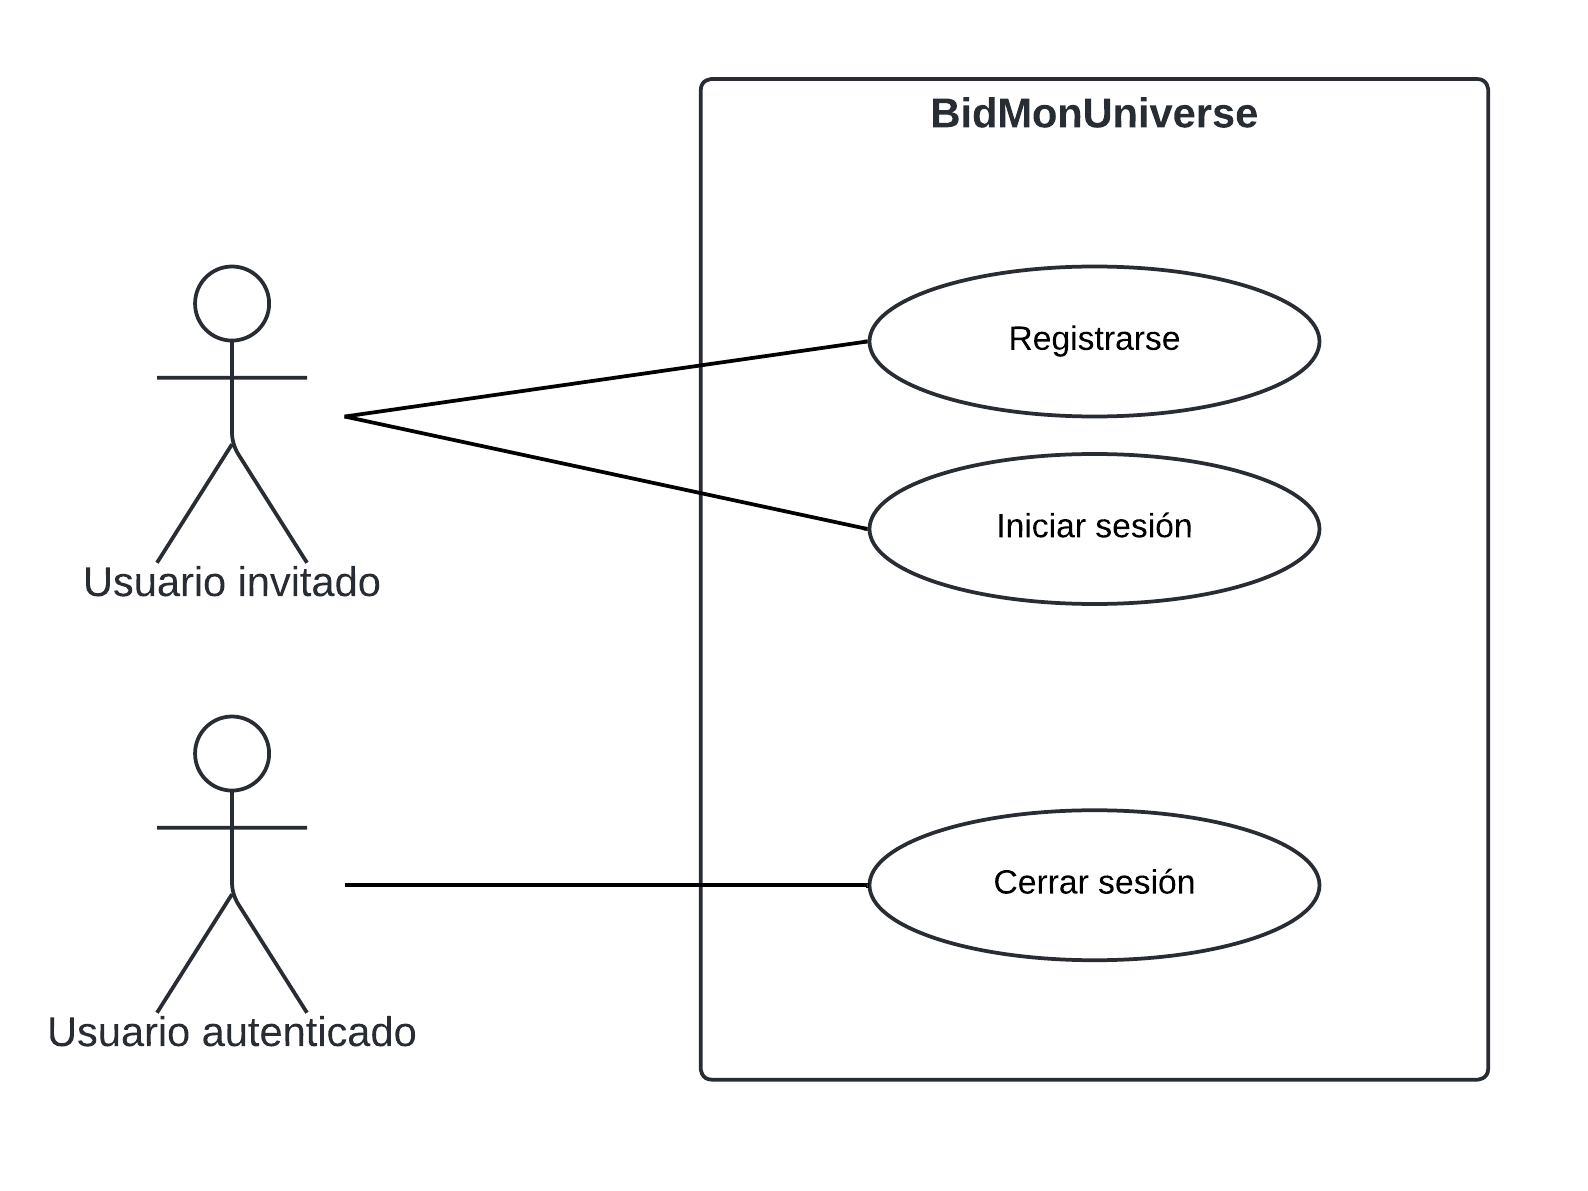
\includegraphics[width=0.5\textwidth]{figures/6-Analisis/6-Casos-uso/6_3_1_Registro-inicio-sesion.png}
    \caption{Casos de uso. Registrarse e iniciar sesión}
    \label{fig:cu_registro-inicio-sesion}
\end{figure}


\subsubsection{Caso de uso. Registrarse} \label{sec:cu_registro}
\begin{longtable}{
    >{\columncolor{lightgreen!20}}p{4cm}
    p{12cm}
    }
    \caption{Caso de uso. Registrarse} \label{table:cu_registro} \\
    \toprule
    \rowcolor{darkgreen!50}
    \textbf{Caso de uso} & \multicolumn{1}{>{\columncolor{darkgreen!50}\centering\arraybackslash}p{12cm}}{\textbf{REGISTRO}} \\
    \endfirsthead
    
    \multicolumn{2}{c}%
    {{ \tablename\ \thetable{} Caso de uso. Registrarse -- continuación de la página anterior}} \\
    \toprule
    \rowcolor{darkgreen!50}
    \textbf{Caso de uso} & \multicolumn{1}{>{\columncolor{darkgreen!50}\centering\arraybackslash}p{12cm}}{\textbf{REGISTRO}} \\
    \midrule
    \endhead
    
    \midrule
    \multicolumn{2}{r}{{Continúa en la siguiente página...}} \\ 
    \endfoot
    
    \bottomrule
    \endlastfoot
    
    \midrule
    Descripción & Un usuario no autenticado se puede registrar en el sistema para poder acceder a las funcionalidades del mismo. \\
    \midrule
    Actores principales & Usuario no autenticado \\
    \midrule
    Actores secundarios &  \\
    \midrule
    Precondiciones & El usuario no debe estar registrado en el sistema. \\
    \midrule
    Postcondiciones & \begin{itemize}[nosep,leftmargin=*]
      \item Se crea un nuevo registro en la base de datos con los datos del usuario.
      \item Se notifica al usuario que su registro ha sido exitoso.
      \item Se redirige al usuario a la página de inicio de sesión.
    \end{itemize} \\
    \midrule
    Disparadores & El usuario hace clic en el botón de registro. \\
    \midrule
    Escenario principal & \begin{enumerate}[nosep,leftmargin=*]
      \item El sistema muestra el formulario de registro.
      \item El usuario completa el formulario con sus datos personales.
      \item El usuario hace clic en el botón de registro.
      \item El sistema valida los datos del formulario.
      \item El sistema crea un nuevo registro en la base de datos con los datos del usuario.
      \item El sistema notifica al usuario que su registro ha sido exitoso.
      \item El sistema redirige al usuario a la página de inicio de sesión.
    \end{enumerate} \\
    \midrule
    Escenarios alternativos & 
    \begin{itemize}[nosep,leftmargin=*]
      \item \textbf{Escenario alternativo 1. El usuario cancela el registro.}
      \begin{enumerate}[nosep,leftmargin=*]
          \item El usuario hace clic en otro enlace.
          \item El sistema no crea el registro y redirige al usuario a la página correspondiente.
      \end{enumerate}
      \item \textbf{Escenario alternativo 2. El usuario ya está registrado en el sistema.}
      \begin{enumerate}[nosep,leftmargin=*]
          \item El sistema muestra un mensaje de error.
          \item El sistema no crea el registro y redirige al usuario de nuevo al formulario de registro.
      \end{enumerate}
      \item \textbf{Escenario alternativo 3. El usuario no completa el formulario correctamente.}
      \begin{enumerate}[nosep,leftmargin=*]
          \item El sistema muestra un mensaje de error con los campos que no se han completado correctamente.
          \item El sistema no crea el registro y redirige al usuario de nuevo al formulario de registro.
      \end{enumerate}
    \end{itemize} \\
    \midrule
    Situaciones de error & \begin{itemize}[nosep,leftmargin=*]
      \item \textbf{Error de conexión a la base de datos.}
      \begin{enumerate}[nosep,leftmargin=*]
          \item El sistema muestra un mensaje de error.
          \item El sistema redirige al usuario de nuevo al formulario de registro.
      \end{enumerate}
    \end{itemize} \\
    \end{longtable}


\subsubsection{Caso de uso. Iniciar sesión} \label{sec:cu_inicio-sesion}
\begin{longtable}{
    >{\columncolor{lightgreen!20}}p{4cm}
    p{12cm}
    }
    \caption{Caso de uso. Iniciar sesión} \label{table:cu_inicio-sesion} \\
    \toprule
    \rowcolor{darkgreen!50}
    \textbf{Caso de uso} & \multicolumn{1}{>{\columncolor{darkgreen!50}\centering\arraybackslash}p{12cm}}{\textbf{INICIAR SESIÓN}} \\
    \endfirsthead
    
    \multicolumn{2}{c}%
    {{ \tablename\ \thetable{} Caso de uso. Iniciar sesión -- continuación de la página anterior}} \\
    \toprule
    \rowcolor{darkgreen!50}
    \textbf{Caso de uso} & \multicolumn{1}{>{\columncolor{darkgreen!50}\centering\arraybackslash}p{12cm}}{\textbf{INICIAR SESIÓN}} \\
    \midrule
    \endhead
    
    \midrule
    \multicolumn{2}{r}{{Continúa en la siguiente página...}} \\ 
    \endfoot
    
    \bottomrule
    \endlastfoot
    
    \midrule
    Descripción & Un usuario no autenticado puede iniciar sesión en el sistema para acceder a las funcionalidades del mismo. \\
    \midrule
    Actores principales & Usuario no autenticado \\
    \midrule
    Actores secundarios &  \\
    \midrule
    Precondiciones & El usuario debe de haberse registrado previamente en el sistema. \\
    \midrule
    Postcondiciones & \begin{itemize}[nosep,leftmargin=*]
        \item Se crea una nueva sesión para el usuario.
        \item Se redirige al usuario a la página de inicio.
    \end{itemize} \\
    \midrule
    Disparadores & El usuario hace clic en el botón de inicio de sesión. \\
    \midrule
    Escenario principal & \begin{enumerate}[nosep,leftmargin=*]
        \item El sistema muestra el formulario de inicio de sesión.
        \item El usuario completa el formulario con sus credenciales.
        \item El usuario hace clic en el botón de inicio de sesión.
        \item El sistema valida las credenciales del usuario.
        \item El sistema crea una nueva sesión para el usuario.
        \item El sistema redirige al usuario a la página de inicio.
    \end{enumerate} \\
    \midrule
    Escenarios alternativos & 
    \begin{itemize}[nosep,leftmargin=*]
      \item \textbf{Escenario alternativo 1. El usuario cancela el inicio de sesión.}
      \begin{enumerate}[nosep,leftmargin=*]
          \item El usuario hace clic en otro enlace.
          \item El sistema no crea la sesión para el usuario y redirige al usuario a la página correspondiente.
      \end{enumerate}
      \item \textbf{Escenario alternativo 2. El usuario no está registrado en el sistema o la contraseña es incorrecta.}
      \begin{enumerate}[nosep,leftmargin=*]
          \item El sistema muestra un mensaje de error.
          \item El sistema no crea la sesión para el usuario y redirige al usuario de nuevo al formulario de inicio de sesión.
      \end{enumerate}
      \item \textbf{Escenario alternativo 3. El usuario no completa el formulario correctamente.}
      \begin{enumerate}[nosep,leftmargin=*]
          \item El sistema muestra un mensaje de error con los campos que no se han completado correctamente.
          \item El sistema no crea la sesión para el usuario y redirige al usuario de nuevo al formulario de inicio de sesión.
      \end{enumerate}
    \end{itemize} \\
    \midrule
    Situaciones de error & \begin{itemize}[nosep,leftmargin=*]
      \item \textbf{Error de conexión a la base de datos.}
      \begin{enumerate}[nosep,leftmargin=*]
          \item El sistema muestra un mensaje de error.
          \item El sistema redirige al usuario de nuevo al formulario de inicio de sesión.
      \end{enumerate}
    \end{itemize} \\
    \end{longtable}


\subsubsection{Caso de uso. Cerrar sesión} \label{sec:cu_cerrar-sesion}
\begin{longtable}{
    >{\columncolor{lightgreen!20}}p{4cm}
    p{12cm}
    }
    \caption{Caso de uso. Cerrar sesión} \label{table:cu_cerrar-sesion} \\
    \toprule
    \rowcolor{darkgreen!50}
    \textbf{Caso de uso} & \multicolumn{1}{>{\columncolor{darkgreen!50}\centering\arraybackslash}p{12cm}}{\textbf{CERRAR SESIÓN}} \\
    \endfirsthead
    
    \multicolumn{2}{c}%
    {{ \tablename\ \thetable{} Caso de uso. Cerrar sesión -- continuación de la página anterior}} \\
    \toprule
    \rowcolor{darkgreen!50}
    \textbf{Caso de uso} & \multicolumn{1}{>{\columncolor{darkgreen!50}\centering\arraybackslash}p{12cm}}{\textbf{CERRAR SESIÓN}} \\
    \midrule
    \endhead
    
    \midrule
    \multicolumn{2}{r}{{Continúa en la siguiente página...}} \\ 
    \endfoot
    
    \bottomrule
    \endlastfoot
    
    \midrule
    Descripción & Un usuario autenticado puede cerrar sesión en el sistema. \\
    \midrule
    Actores principales & Usuario autenticado \\
    \midrule
    Actores secundarios &  \\
    \midrule
    Precondiciones & El usuario debe de haber iniciado sesión previamente en el sistema. \\
    \midrule
    Postcondiciones & \begin{itemize}[nosep,leftmargin=*]
        \item Se elimina la sesión del usuario.
    \end{itemize} \\
    \midrule
    Disparadores & El usuario hace clic en el botón de cerrar sesión. \\
    \midrule
    Escenario principal & \begin{enumerate}[nosep,leftmargin=*]
        \item El sistema muestra la opción de cerrar sesión.
        \item El usuario hace clic en el botón de cerrar sesión.
        \item El sistema elimina la sesión del usuario.
        \item El sistema redirige al usuario a la página de inicio.
    \end{enumerate} \\
    \midrule
    Escenarios alternativos & \\
    \midrule
    Situaciones de error & \\
    \end{longtable}